\documentclass[11pt]{article}
% BAI (Biblioteca de Autorização Isomórfica) + profundidade δ — broca-so / conversa Tiffany
\usepackage[utf8]{inputenc}
\usepackage[T1]{fontenc}
\usepackage[brazil]{babel}
\usepackage{amsmath,amssymb,amsthm}
\usepackage{libertinus-type1}
\usepackage{libertinust1math}
\usepackage[margin=3.2cm]{geometry}
\usepackage{mathtools}
\usepackage{stmaryrd}
\usepackage{enumitem}
\usepackage{array}
\usepackage{booktabs}
\usepackage{hyperref}
\usepackage{graphicx}
\usepackage{xcolor}
\usepackage{eso-pic}
\usepackage{titlesec}
\usepackage{pifont}
\usepackage{tikz}
\usetikzlibrary{trees,positioning,fit,backgrounds,calc,arrows.meta}
\usepackage[framemethod=default]{mdframed}
\setlength{\abovedisplayskip}{13pt}\setlength{\belowdisplayskip}{13pt}

\definecolor{creme}{HTML}{F8F5EE}
\definecolor{ouro}{HTML}{8B6914}
\definecolor{ourovivo}{HTML}{B8860B}
\definecolor{prata}{HTML}{6E7681}
\definecolor{tinta}{HTML}{2A2623}
\pagecolor{creme}\color{tinta}
\renewcommand{\thesection}{\Roman{section}}
\titleformat{\section}[display]
  {\centering\normalfont}
  {\textcolor{ourovivo}{\ding{117}}\\[1pt]{\color{prata}\scshape\normalsize\thesection}}
  {1pt}{\color{ouro}\scshape\Large}
\titlespacing*{\section}{0pt}{1.7em}{0.9em}
\newcommand{\est}[1]{\textsf{\footnotesize[#1]}}
\newcommand{\SO}{\textsc{Broca\,OS}}
\newcommand{\Tiffany}{\textsc{Tiffany}}
\newcommand{\BAI}{\textsc{Biblioteca de Autorização Isomórfica}}

\hypersetup{colorlinks=true,linkcolor=ourovivo,urlcolor=ourovivo,citecolor=prata}

\newtheorem{theorem}{Teorema}
\newtheorem{lemma}[theorem]{Lema}
\newtheorem{corollary}[theorem]{Corolário}
\newtheorem{proposition}[theorem]{Proposição}
\theoremstyle{definition}
\newtheorem{definition}[theorem]{Definição}
\newtheorem{remark}[theorem]{Observação}
\surroundwithmdframed[topline=false,bottomline=false,rightline=false,linecolor=ourovivo,
  linewidth=1.8pt,leftmargin=0pt,innerleftmargin=12pt,innertopmargin=2pt,innerbottommargin=4pt,
  backgroundcolor=creme,skipabove=10pt,skipbelow=8pt]{proposition}
\surroundwithmdframed[topline=false,bottomline=false,rightline=false,linecolor=ouro,
  linewidth=2.8pt,leftmargin=0pt,innerleftmargin=12pt,innertopmargin=2pt,innerbottommargin=4pt,
  backgroundcolor=creme,skipabove=10pt,skipbelow=8pt]{theorem}
\surroundwithmdframed[topline=false,bottomline=false,rightline=false,linecolor=prata,
  linewidth=1.4pt,leftmargin=0pt,innerleftmargin=12pt,innertopmargin=2pt,innerbottommargin=4pt,
  backgroundcolor=creme,skipabove=8pt,skipbelow=6pt]{definition}
\newmdenv[topline=false,bottomline=false,rightline=false,linecolor=prata!80,
  linewidth=1.1pt,leftmargin=0pt,innerleftmargin=11pt,innertopmargin=3pt,innerbottommargin=5pt,
  backgroundcolor=creme!92!prata!8,skipabove=6pt,skipbelow=6pt]{engimpl}
\newcommand{\eng}[1]{\begin{engimpl}\small\textsc{Nota de engenharia.}\ #1\end{engimpl}}

\AddToShipoutPictureBG{%
  \IfFileExists{arvore_metais.pdf}{%
    \put(0,0){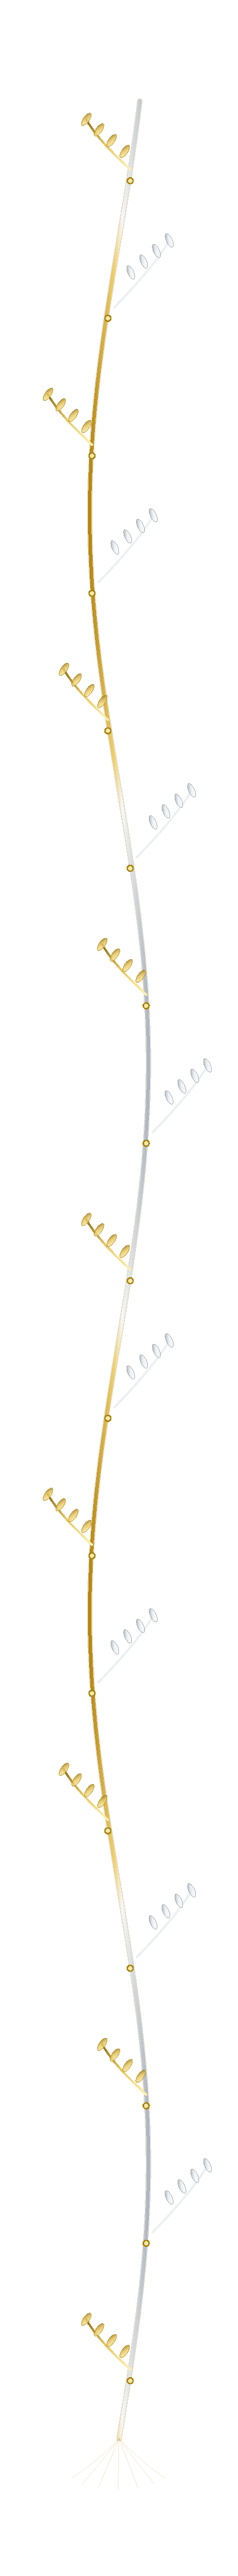
\includegraphics[height=\paperheight]{arvore_metais.pdf}}%
    \put(\dimexpr\paperwidth-78pt\relax,0){\reflectbox{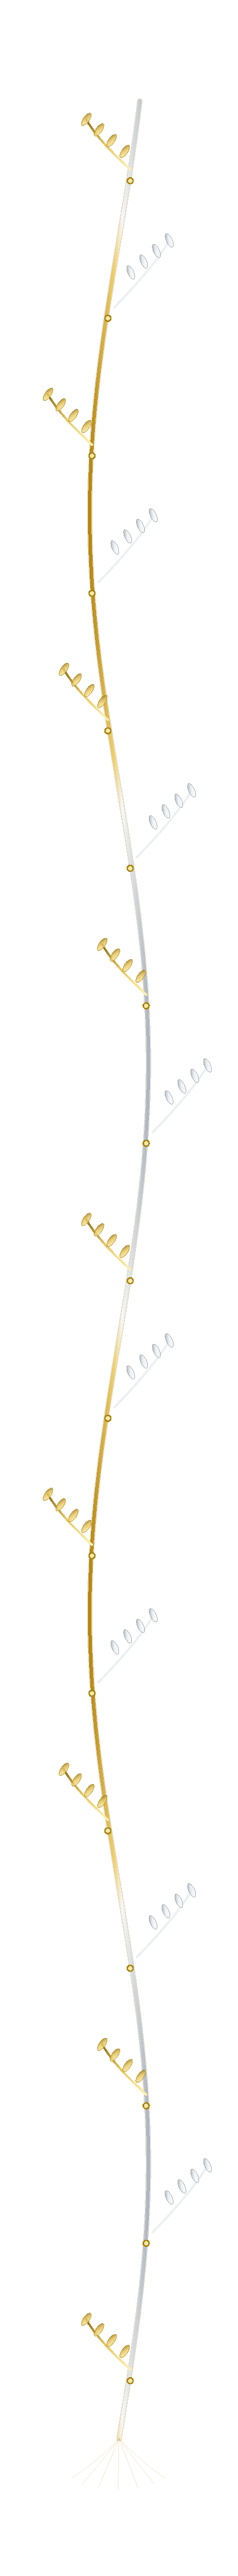
\includegraphics[height=\paperheight]{arvore_metais.pdf}}}%
  }{}%
}

\newcommand{\R}{\mathcal{R}}
\newcommand{\ext}[1]{\llbracket #1 \rrbracket}
\newcommand{\Subj}{\mathcal{S}}
\newcommand{\Act}{\mathcal{A}}
\newcommand{\tenant}{\texttt{tenantId}}
\newcommand{\dep}{\delta}
\newcommand{\NN}{\mathbb{N}_0}
\newcommand{\F}{\mathcal{F}}
\newcommand{\dS}{\mathrm{dS}}
\newcommand{\CalC}{\mathcal{C}}
\newcommand{\Collapse}{\mathrm{Collapse}}
\newcommand{\Phif}{\Phi}

\newcommand{\parttitle}[1]{%
  \clearpage
  \vspace*{0.5em}
  \begin{center}
  {\color{ourovivo}\rule{2.4cm}{0.5pt}}\\[6pt]
  {\fontsize{15}{18}\selectfont\scshape\color{ouro}#1}\\[6pt]
  {\color{prata}\rule{2.4cm}{0.5pt}}
  \end{center}
  \vspace{1.2em}
}

\title{\vspace{-2.4cm}
\IfFileExists{logo_moeda.png}{
\includegraphics[width=0.184\textwidth]{logo_moeda.png}\\[10pt]}{}
{\color{ourovivo}\rule{1.6cm}{0.5pt}}{\color{prata}\rule{1.6cm}{0.5pt}}\\[10pt]
{\fontsize{22}{26}\selectfont\scshape\color{ouro}Biblioteca de Autorização Isomórfica}\\[8pt]
{\fontsize{13}{17}\selectfont\scshape\color{tinta!78}propagação, atenuação e colapso --- $\dep$ e $\Phif$ como primitivas}\\[2pt]}
\author{\normalsize Aarão Melo Lopes \quad\textit{\color{prata}(com Claude)}}
\date{\small\color{prata} Junho de 2026 \;\textbullet\; documento vivo}

\begin{document}
\maketitle
\thispagestyle{empty}

\begin{center}
{\large\itshape\color{tinta!85}Uma biblioteca matemática de propagação e atenuação. CASL, \SO\ e \Tiffany\ são instâncias --- não motivações.}
\end{center}

\bigskip

\begin{abstract}
\noindent
Apresentamos a \BAI: biblioteca de \emph{delegação capacitária} sobre reticulados
booleanos. Primitivas: \textbf{capacidade} $\kappa=(\sigma,c,\dep,\omega,o)$,
\textbf{orçamento} $\dep\in\NN\cup\{\infty\}$ (propagação discreta),
\textbf{par} $(\Phif,\dep)$ (estrutura vs.\ alcance), operadores $T\preceq\mathrm{id}$
(atenuação), $P\succeq\mathrm{id}$ (propagação) e \textbf{colapso}
$\Psi=\Collapse(\CalC_\dep)$ sobre candidatos vigentes $\CalC_\dep=\{\kappa:\dep>0\}$.
Teoremas: não-escalada, propagação limitada, fail-closed --- independentes de
domínio. Toda instância é determinada pelo quinteto
$(\kappa,\dep,\Phif,T,\Psi)$; CASL, \SO\ e \Tiffany\ são interpretações.
\textbf{Parte~II--IV} instanciam; analogias físicas ficam no Apêndice.
\end{abstract}

\begin{center}\small\scshape\color{prata}
$\CalC_\dep$ \textcolor{ourovivo}{\footnotesize\ding{117}}\ $\Psi=\Collapse$ \textcolor{ourovivo}{\footnotesize\ding{117}}
$(\Phif,\dep)$ \textcolor{ourovivo}{\footnotesize\ding{117}}\ $T\preceq\mathrm{id}$ \textcolor{ourovivo}{\footnotesize\ding{117}}\ fail-closed
\end{center}

\bigskip

\parttitle{Parte I --- Biblioteca matemática}

% ============================================================
\section{Introdução}
% ============================================================

\est{L} Este documento apresenta uma \emph{biblioteca} --- não uma aplicação.
Autoridade flui, atenua ($T\preceq\mathrm{id}$), propaga com orçamento $\dep$,
organiza-se ($\Phif$) e colapsa ($\Psi$) ou falha fechada ($\varnothing$).

\begin{theorem}[Tese-mãe da \BAI]\label{thm:mae}
Toda instância da \emph{Biblioteca de Autorização Isomórfica} é determinada
pelo \textbf{quinteto}
\[
  (\kappa,\,\dep,\,\Phif,\,T,\,\Psi),
\]
onde $\kappa$ é capacidade abstrata (Definição~\ref{def:kappa-abstract}),
$\dep$ orçamento de propagação (Definição~\ref{def:delta-budget}),
$\Phif$ medida de organização estrutural (Definição~\ref{def:phi-abstract}),
$T$ operador de atenuação deflacionário e $\Psi$ operador de colapso
(Definições~\ref{def:TP} e~\ref{def:collapse}). CASL, \SO\ e \Tiffany\
são \emph{interpretações} distintas destas primitivas --- não motivações
do formalismo (Seção~\ref{ap:iso}).
\end{theorem}

% ============================================================
\section{Capacidade abstrata}\label{sec:kappa}
% ============================================================

\begin{definition}[Universo e extent]\label{def:universo}
Fixe um universo $X$. Uma \emph{condição} $c$ é um predicado
$c:X\to\{\bot,\top\}$, identificado ao \emph{extent}
$\ext{c}\subseteq X$. As condições formam o reticulado booleano
$(2^X,\cup,\cap,\setminus,\varnothing,X)$.
\end{definition}

\begin{definition}[Capacidade]\label{def:kappa-abstract}
Uma \emph{capacidade} é uma tupla
\[
  \kappa=(\sigma,\,c,\,\dep,\,\omega,\,o),
  \qquad \dep\in\NN\cup\{\infty\},
\]
onde $\sigma$ é o \emph{estado}, $c$ a condição,
$\dep$ o orçamento (Seção~\ref{sec:delta}), $\omega$ o peso
(grant/deny quando aplicável) e $o$ a origem. Nenhum domínio entra na
definição.
\end{definition}

\begin{remark}[Instanciações]\label{rem:instancias}
Parte~II: $\sigma=(a,s)$, $\omega\leftrightarrow\iota$. Parte~III: $\sigma$
é identificador de nó no tecido. Parte~IV: $\sigma$ é um turno dialogado
\texttt{A — B}.
\end{remark}

% ============================================================
\section{Orçamento $\dep$}\label{sec:delta}
% ============================================================

\begin{definition}[Orçamento de propagação]\label{def:delta-budget}
$\dep$ representa um \textbf{orçamento discreto de propagação}: quantas
re-delegações (saltos, turnos, réplicas) a capacidade ainda admite.
$\dep=0$ --- usa mas não repassa; $\dep=k$ --- mais $k$ saltos, decrementando;
$\dep=\infty$ --- fecho transitivo ($\mu P$). A verificação de $\dep$ ocorre
no \emph{ato de delegar}, nunca na avaliação/colapso.
\end{definition}

\begin{remark}[Leituras por domínio --- sem alterar a definição]
\begin{center}\small
\begin{tabular}{@{}ll@{}}
CASL & re-delegação de permissões \\
conversa / memória & profundidade de cadeia ou persistência \\
replicação & alcance em grafo distribuído \\
\end{tabular}
\end{center}
\end{remark}

% ============================================================
\section{Organização estrutural $\Phif$}\label{sec:phi}
% ============================================================

\begin{definition}[Medida $\Phif$]\label{def:phi-abstract}
Fixe um espaço de estados $\mathcal{S}$ (configurações, impressões, snapshots).
Uma \textbf{medida de organização estrutural} é um funcional
\[
  \Phif:\mathcal{S}\longrightarrow \mathbb{R}_{\ge 0}\cup\{\top\},
\]
monótono sob agregação observável: estados mais estruturados (menos
dispersos, mais estáveis sob transformação) carregam $\Phif$ mais
informativo. $\Phif$ não entra no colapso $\Psi$ --- observa o \emph{efeito}
da propagação/atenuação, complementar a $\dep$.
\end{definition}

\begin{remark}[Métricas por domínio]\label{rem:phi-metrics}
Cada instância escolhe sua métrica concreta de $\Phif$:
\begin{center}\small
\begin{tabular}{@{}ll@{}}
CASL & entropia de políticas, cardinalidade de grants ativos \\
\SO & dissipação não-associativa acumulada (recipiente) \\
\Tiffany & frames, atratores únicos, bits de estabilidade por turno \\
\end{tabular}
\end{center}
\end{remark}

% ============================================================
\section{Par fundacional $(\Phif,\dep)$}\label{sec:phi-delta}
% ============================================================

\begin{definition}[Par $(\Phif,\dep)$]\label{def:phi-delta}
$\dep$ \textbf{controla propagação} (alcance, saltos restantes).
$\Phif$ \textbf{controla estabilidade observável} (organização estrutural
do estado). Diálogos ou delegações longas consomem $\dep$ e, em geral,
aumentam $\Phif$ --- mais estrutura acumulada --- sem violar atenuação.
\end{definition}

\begin{remark}[Associativo \emph{vs.} estrutural]
Em instâncias com endereçamento associativo (overlap, extent SQL), $\Psi$
opera sobre o associativo; $\Phif$ captura o que o endereçamento não
conserva. Os dois eixos são independentes por construção.
\end{remark}

% ============================================================
\section{Operadores $T$, $P$ e colapso $\Psi$}\label{sec:TP-collapse}
% ============================================================

\begin{definition}[Atenuação e propagação]\label{def:TP}
Sobre extents: $T:2^X\to2^X$ é \textbf{monótono deflacionário}
($T\preceq\mathrm{id}$, $x\subseteq y\Rightarrow T(x)\subseteq T(y)$).
Sobre detentores: $P:2^{\hat P}\to2^{\hat P}$ é \textbf{monótono inflacionário}
($P\succeq\mathrm{id}$). Re-delegar por $\dep$ saltos é $P^{\dep}$;
$\dep=\infty$ corresponde ao menor ponto fixo $\mu P=\bigsqcup_n P^n(H_0)$.
\end{definition}

\begin{definition}[Conjunto vigente e colapso $\Psi$]\label{def:collapse}
Seja $\CalC=\{\kappa_i\}$ capacidades detidas, filtradas por vigência e por
$\ext{c_i}\cap\ext{q}\neq\varnothing$ para consulta $q$. Defina
\[
  \CalC_\dep=\{\kappa\in\CalC:\dep_\kappa>0\ \text{ ou avaliação local}\},
  \qquad
  \Psi(q)=\Collapse(\CalC_\dep,q)
  =\arg\max_{\kappa\in\CalC_\dep}\mathrm{score}(\kappa,q)
\]
(quando o máximo existe; senão $\Psi(q)=\bot$ --- \emph{fail-closed}).
$\Collapse$ é \emph{independente} de $\dep$ restante na leitura: $\dep$ só
entra na formação de $\CalC$ via delegação prévia.
\end{definition}

\begin{theorem}[Universalidade da \BAI]\label{thm:universalidade}
Qualquer sistema cuja autoridade satisfaça:
\begin{enumerate}[nosep,label=(\roman*)]
  \item estados e condições formam um reticulado booleano $(2^X,\cup,\cap)$;
  \item existe operador de atenuação $T\preceq\mathrm{id}$ sobre extents;
  \item existe operador de propagação $P\succeq\mathrm{id}$ com orçamento
        $\dep\in\NN\cup\{\infty\}$ decrementado a cada delegação válida;
  \item existe colapso $\Psi=\Collapse(\CalC_\dep,\cdot)$ sobre candidatos
        vigentes, com fail-closed em $\bot$;
\end{enumerate}
admite uma \textbf{instanciação} na \BAI\ --- isto é, capacidades $\kappa$,
quinteto $(\kappa,\dep,\Phif,T,\Psi)$ e teoremas de não-escalada,
propagação limitada e deny-overrides como corolários da monotonicidade.
\end{theorem}

\begin{proof}[Esboço]
Itens (i)--(iv) são exatamente as hipóteses das Definições~\ref{def:universo},
\ref{def:TP} e~\ref{def:collapse}. Mapear estados para $\sigma$, extents para
$c$, delegações para arestas com $\dep$ decrementado, e avaliação para $\Psi$.
Não-escalada vem de $T\preceq\mathrm{id}$; propagação limitada de $\dep$ como
variante bem-fundada; fail-closed de $\bot$ ser o neutro de $\cup$.
\end{proof}

\parttitle{Parte II --- Instanciação CASL}

% ============================================================
\section{Preliminares CASL}
% ============================================================

\begin{definition}[Linhas e condições]
Seja $\R$ o universo de todas as linhas. Cada $r\in\R$ tem atributos
($r.\tenant$, $r.\texttt{id}$, \dots). Uma \emph{condição} $c$ é um predicado
$c:\R\to\{\bot,\top\}$, identificado ao seu \emph{extent}
$\ext{c}=\{r\in\R:c(r)\}\subseteq\R$. As condições formam a álgebra booleana
$(2^{\R},\cap,\cup,\setminus,\varnothing,\R)$ --- as \emph{MongoQuery} do CASL.
\end{definition}

\begin{remark}[Identificação semântica --- nunca sintática]\label{rem:extent}
Toda \emph{MongoQuery} é identificada ao seu \emph{extent}: os construtores
sintáticos do CASL mapeiam-se nas operações da álgebra,
\[
  \ext{\{\texttt{AND}{:}[c_1,c_2]\}}=\ext{c_1}\cap\ext{c_2},\quad
  \ext{\{\texttt{OR}{:}[c_1,c_2]\}}=\ext{c_1}\cup\ext{c_2},\quad
  \ext{\{\texttt{NOT}{:}c\}}=\R\setminus\ext{c}.
\]
Raciocinamos sempre sobre \emph{conjuntos de linhas}, jamais sobre a forma
da query --- duas queries sintaticamente distintas com o mesmo extent são,
para nós, a \emph{mesma} condição. (Isto não trivializa a implementação: o
teste de inclusão $\subseteq$ no \emph{grant-check} é conservador justamente
porque decidir $\subseteq$ sintaticamente é incompleto; ver
Seção~\ref{sec:enf}.)
\end{remark}

Fixamos \emph{subjects} $\Subj$ (\texttt{Customer}, \texttt{Student}, \dots),
\emph{ações} $\Act=\{\texttt{create},\texttt{read},\texttt{update},
\texttt{delete}\}$ ($\texttt{manage}=\bigvee\Act$) e o curinga \texttt{all}.

\begin{definition}[Capacidade CASL]\label{def:cap}
Specialização da Definição~\ref{def:kappa-abstract} com $X=\R$ (linhas),
$\sigma=(a,s)$ (ação e subject), $\omega\leftrightarrow\iota$ ($\iota{=}1$ é
proibição, \texttt{cannot}) e $\dep$ como orçamento
(Definição~\ref{def:delta-budget}). Formalmente
\[
  \kappa=(a,\,s,\,c,\,\iota,\,\dep), \qquad
  \dep\in\NN\cup\{\infty\},
\]
$\kappa$ autoriza (ou nega, se $\iota{=}1$) $a$ sobre $s$ nas linhas de
$\ext{c}$, e admite re-delegação conforme $\dep$.
\end{definition}

% ============================================================
\section{Autorização de um principal}
% ============================================================

Seja $P$ o conjunto de \emph{principals} (operador, donos de \emph{tenant},
perfis, usuários). Cada principal \emph{detém} um conjunto de capacidades
$\mathrm{Hold}(p)$ (Seção~\ref{sec:dag}). Para um par fixo $(s,a)$, a
autorização efetiva é a \textbf{união} dos grants menos as proibições:
\[
  E_p(s,a)\;=\;
  \Bigl(\bigcup_{\substack{\kappa\in\mathrm{Hold}(p)\\ \iota_\kappa=0,\ \kappa\vdash(s,a)}}\ext{c_\kappa}\Bigr)
  \ \setminus\
  \Bigl(\bigcup_{\substack{\kappa\in\mathrm{Hold}(p)\\ \iota_\kappa=1,\ \kappa\vdash(s,a)}}\ext{c_\kappa}\Bigr),
\]
onde $\kappa\vdash(s,a)$ significa que $\kappa$ casa o subject e a ação
(com \texttt{manage}/\texttt{all} como curingas).

\begin{remark}[A intensidade não entra aqui]
$E_p$ \emph{não} depende de $\dep$: a profundidade governa a \emph{delegação}
(Seção~\ref{sec:dag}), não a avaliação. Quem detém uma capacidade a exerce
plenamente, qualquer que seja o seu $\dep$ restante. Isso é o que torna o
\emph{enforcement} barato (Seção~\ref{sec:enf}).
\end{remark}

\begin{remark}[União, não interseção]
Compor grants com interseção seria um erro: ``ler onde \texttt{org}$=A$'' e
``ler onde \texttt{org}$=B$'' devem autorizar $A\cup B$. Só as proibições
subtraem.
\end{remark}

\begin{proposition}[\emph{Deny-overrides} --- a proibição sempre vence]
\label{prop:deny}
A escolha de política está \emph{embutida} na diferença de conjuntos: para
toda linha $r$,
\[
  r\in E_p(s,a)\iff
  \bigl(\exists\,\text{grant }g:\ r\in\ext{c_g}\bigr)\ \wedge\
  \bigl(\nexists\,\text{proibição }d:\ r\in\ext{c_d}\bigr).
\]
Uma proibição domina \emph{qualquer} grant sobre a mesma linha,
independentemente de ``especificidade'' ou ordem. Assim, grant
$\{\texttt{customerId}{=}5\}$ com proibição $\{\tenant{=}A\}$ (e $5\in A$)
resulta $\varnothing$: a proibição vence. O sistema é, por definição,
\textbf{deny-overrides} --- declarado aqui para remover ambiguidade. (Casa
com a semântica do CASL, onde \texttt{cannot} sobrepõe \texttt{can}.)
\end{proposition}

% ============================================================
\section{O grafo de delegação e a atenuação}\label{sec:dag}
% ============================================================

\begin{definition}[Autoridades intrínsecas]
Duas fontes de autoridade não derivam de ninguém:
\begin{itemize}[nosep]
  \item o \textbf{operador} $\Omega$ detém $(\texttt{manage},\texttt{all},
        \top,0,\infty)$ --- vê e faz tudo, com re-delegação irrestrita;
  \item o \textbf{dono do \emph{tenant}} $t$ detém
        $(\texttt{manage},\texttt{all},(\tenant{=}t),0,\infty)$ --- controle
        total dos próprios recursos.
\end{itemize}
\end{definition}

\begin{definition}[Grafo de delegação]\label{def:dag}
Um \emph{grafo de delegação} é um \emph{grafo dirigido finito} (não
necessariamente acíclico) cujos vértices são principals e cujas arestas
$u\xrightarrow{\kappa}w$ representam ``$u$ concede a capacidade $\kappa$ a
$w$''. $w$ é \emph{qualquer} principal --- sem exigência de árvore, de
vizinhança ou de aciclicidade.
\end{definition}

\begin{definition}[Concessão válida / atenuação]\label{def:att}
A aresta $u\xrightarrow{\kappa}w$ é \emph{válida} se existe
$\kappa_0\in\mathrm{Hold}(u)$ tal que
\[
  \ext{c_\kappa}\subseteq\ext{c_{\kappa_0}},\quad
  \kappa\vdash(s,a)\Rightarrow\kappa_0\vdash(s,a),\quad
  \iota_\kappa=\iota_{\kappa_0},\quad
  \dep_{\kappa_0}\ge 1,\quad
  \dep_\kappa\le \dep_{\kappa_0}-1,\quad
  \tau_\kappa\le\tau_{\kappa_0},
\]
com a convenção $\infty-1=\infty$. Isto é, $u$ só concede o que detém,
\emph{nunca ampliando} a condição, \emph{sempre decrementando} a
profundidade e \emph{nunca estendendo} a validade $\tau$ (expiração,
Seção~\ref{sec:lifecycle}). Em particular $\dep_{\kappa_0}=0$ proíbe qualquer
concessão.
\end{definition}

\begin{definition}[Capacidades detidas]
$\mathrm{Hold}(p)$ é o menor conjunto que contém as capacidades intrínsecas
de $p$ (se $p$ é $\Omega$ ou dono) e toda $\kappa$ tal que existe uma aresta
válida $u\xrightarrow{\kappa}p$.
\end{definition}

% ------------------------------------------------------------
\subsection{A intensidade $\dep$: profundidade de propagação}
% ------------------------------------------------------------

Por construção (Definição~\ref{def:att}), uma capacidade emitida com
profundidade $\dep$ admite cadeias de re-delegação de comprimento no máximo
$\dep$:
\[
  \dep \xrightarrow{\text{1 salto}} \dep-1 \xrightarrow{} \cdots \xrightarrow{} 0
  \ (\text{não re-delegável}).
\]
\begin{itemize}[nosep]
  \item $\dep=0$: o destinatário \emph{usa} a capacidade, mas não a passa a
        ninguém. É o caso do ``dar acesso sem permitir compartilhar''.
  \item $\dep=k$: re-delegável por mais $k$ saltos; cada salto decrementa.
  \item $\dep=\infty$: irrestrito (o comportamento legado, sem limite).
\end{itemize}

\begin{lemma}[$\dep$ é uma energia bem-fundada $\Rightarrow$ ciclos são inofensivos]
\label{lem:energy}
Como toda aresta válida \emph{estritamente} decrementa a profundidade
($\dep_\kappa\le\dep_{\kappa_0}-1$, Definição~\ref{def:att}), $\dep$ é um
\emph{variante bem-fundado} sobre as cadeias de re-delegação: qualquer
caminho de concessões com $\dep$ finito tem comprimento $\le\dep$ e termina.
\textbf{Logo a aciclicidade do grafo é dispensável} --- um ciclo
$u\to v\to\cdots\to u$ apenas faz $\dep$ cair a cada volta até $0$, quando a
propagação para. A terminação (e a não-escalada) vem da atenuação, não da
estrutura do grafo. Só $\dep=\infty$ ignora a energia; reserve-o às
autoridades intrínsecas.
\end{lemma}

  \begin{figure}[h]
  \centering
  \begin{tikzpicture}[
      every node/.style={font=\small},
      P/.style={draw=ourovivo,circle,inner sep=2pt,fill=creme,minimum size=8mm},
      dlbl/.style={midway,font=\scriptsize,text=tinta!70,align=center},
      >={Stealth[round]},
    ]
  \node[P] (op) {$\Omega$};
  \node[P, below=14mm of op] (ad) {A};
  \node[P, below left=16mm and 10mm of ad] (u1) {$u_1$};
  \node[P, below right=16mm and 10mm of ad] (u2) {$u_2$};
  \node[P, below=14mm of u1] (u3) {$u_3$};

  % delegação intrínseca e cross-tenant com profundidade
  \draw[->] (op) -- (ad) node[dlbl,right]{cross-tenant\\ $(\tenant{=}B,\ \dep{=}1)$};
  \draw[->] (ad) -- (u1) node[dlbl,left]{$\dep{=}0$};
  \draw[->,dashed,gray] (u1) -- (u3) node[dlbl,left]{\textcolor{red!70!black}{bloqueada}\\ $\dep{=}0$};
  \draw[->] (ad) -- (u2) node[dlbl,right]{interno A\\ $(\tenant{=}A,\ \dep{=}0)$};
\end{tikzpicture}
\caption{Grafo de delegação (dirigido finito, não árvore, ciclos permitidos). $\Omega$ concede a $A$ uma
capacidade cross-\emph{tenant} ($\tenant{=}B$) com $\dep{=}1$; $A$ pode
re-delegá-la \emph{uma} vez (a $u_1$, com $\dep{=}0$), mas $u_1$ \emph{não}
pode repassá-la (aresta bloqueada). $A$ também concede algo interno
diretamente a $u_2$. As arestas são explícitas --- $A$ alcança $u_1,u_2$
diretamente, sem intermediários obrigatórios.}
\label{fig:dag}
\end{figure}

% ============================================================
\section{Invariantes de segurança}
% ============================================================

\begin{theorem}[Não-escalada por atenuação]\label{thm:noesc}
Para todo $p$ e toda $\kappa\in\mathrm{Hold}(p)$, existe uma autoridade
intrínseca $\kappa_0$ e uma cadeia de arestas válidas de sua origem até $p$
tais que $\ext{c_\kappa}\subseteq\ext{c_{\kappa_0}}$. Logo
\[
  E_p(s,a)\ \subseteq\ \bigcup_{\kappa_0\ \text{(raiz que alcança }p)}\ext{c_{\kappa_0}} .
\]
Nenhum principal acessa uma linha que nenhuma autoridade intrínseca em sua
cadeia podia conceder.
\end{theorem}
\begin{proof}
Indução no comprimento da cadeia de delegação. Caso base: capacidade
intrínseca. Passo: a Definição~\ref{def:att} exige
$\ext{c_\kappa}\subseteq\ext{c_{\kappa_0}}$ a cada aresta; a inclusão é
transitiva. A cota de $E_p$ segue por monotonicidade da união.
\end{proof}

\begin{theorem}[Propagação limitada]\label{thm:bounded}
Uma capacidade emitida com profundidade $\dep$ só pode aparecer (atenuada)
ao fim de cadeias de re-delegação de comprimento $\le\dep$. Em particular,
$\dep=0\Rightarrow$ não re-delegável: ela permanece exclusivamente no
destinatário direto.
\end{theorem}
\begin{proof}
Cada aresta válida decrementa $\dep$ em pelo menos 1 e exige $\dep_{\kappa_0}
\ge1$ (Definição~\ref{def:att}); uma cadeia de comprimento $\ell$ requer
$\dep\ge\ell$. Para $\dep=0$ não há aresta de saída possível.
\end{proof}

\begin{corollary}[Compartilhamento controlado]
Conceder uma capacidade cross-\emph{tenant} com $\dep=0$ garante que o
destinatário a exerce mas ninguém abaixo dele a herda --- exatamente ``dar
acesso sem propagar''. Com $\dep=k$, a difusão é confinada à vizinhança de
re-delegação de raio $k$.
\end{corollary}

\begin{remark}[Fail-closed $=$ união vazia]
Se nenhum grant detido casa $(s,a)$, então $E_p(s,a)=\varnothing$: acesso
negado. É o \emph{bottom} da álgebra, uniforme --- sem piso de tenant
especial.
\end{remark}

% ============================================================
\section{O tenant como caso particular (desacoplamento)}
% ============================================================

\begin{corollary}[Isolamento de tenant]
Um usuário comum da organização $t$ só detém capacidades atenuadas da
capacidade intrínseca do dono, todas com $\ext{c}\subseteq\ext{\tenant{=}t}$.
Logo $E_p\subseteq\{r:r.\tenant=t\}$: nenhuma linha de outro \emph{tenant}
aparece, \emph{sem} regra especial. Um vazamento cross-\emph{tenant} só
ocorre por uma aresta de concessão explícita (auditável), cuja difusão é
exatamente governada por $\dep$.
\end{corollary}

O operador $\Omega$, detendo $\top$, enxerga todos os \emph{tenants} --- ``eu,
no topo, vejo tudo''. O \emph{tenant} foi reduzido a uma condição.

% ============================================================
\section{Caracterização algébrica}\label{sec:algebra}
% ============================================================

Tudo o que precede é, na verdade, \emph{um fluxo monótono sobre um reticulado
booleano}. Tornar isso explícito entrega vários teoremas quase de graça.

\begin{definition}[O dioid das condições]
$(2^{\R},\oplus,\otimes)$ com $\oplus:=\cup$ e $\otimes:=\cap$ é um
\emph{semianel idempotente comutativo} (dioid): $\oplus$ é associativa,
comutativa, \emph{idempotente} ($a\oplus a=a$), com neutro $\varnothing$;
$\otimes$ idem, com neutro $\R$; e $\otimes$ distribui sobre $\oplus$. A
\emph{ordem canônica} $a\preceq b\iff a\oplus b=b$ coincide com $\subseteq$.
Com o complemento $\neg$, é a álgebra booleana completa
$(2^{\R},\cup,\cap,\neg,\varnothing,\R)$ --- um \emph{reticulado completo}.
\end{definition}

\begin{remark}[Autorização é uma expressão do dioid]
A Seção~3 é, literalmente, álgebra do semianel:
\[
  E_p(s,a)=\Bigl(\bigoplus_{g}\ext{c_g}\Bigr)\otimes
          \neg\Bigl(\bigoplus_{n}\ext{c_n}\Bigr),
\]
soma dos grants vezes o complemento da soma das proibições. O
\emph{pushdown} (Seção~\ref{sec:enf}) é apenas avaliar essa expressão.
\end{remark}

\begin{definition}[Delegação é um operador monótono deflacionário]
Cada aresta de delegação induz $T:2^{\R}\to2^{\R}$ com
\[
  x\preceq y\Rightarrow T(x)\preceq T(y)\quad(\text{monótono}),\qquad
  T(x)\preceq x\quad(\text{deflação: }T\preceq\mathrm{id}).
\]
A condição de atenuação $\ext{c_\kappa}\subseteq\ext{c_{\kappa_0}}$
(Definição~\ref{def:att}) \emph{é} exatamente $T\preceq\mathrm{id}$.
\end{definition}

\paragraph{Dois operadores duais (a distinção que importa).}
A delegação tem \emph{dois} lados, e é tentador --- mas incorreto --- fundir
os dois. A \textbf{atenuação} $T\preceq\mathrm{id}$ (deflacionária, sobre os
extents $2^{\R}$) governa \emph{o que}: o extent só encolhe. A
\textbf{propagação} $P$ governa \emph{quem detém}: sobre o reticulado
completo $2^{\hat P}$ dos conjuntos de principals,
\[
  P(H)=H\cup\{\,w:\exists\,u\in H,\ \text{aresta válida }u\to w\,\},
  \qquad P\succeq\mathrm{id}\ (\text{inflacionária}),\ \text{monótona}.
\]

\paragraph{Os resultados de graça.}
\begin{itemize}[nosep,leftmargin=1.3em]
  \item \textbf{Profundidade $=$ iteração da propagação $P$ (não de $T$).}
        Re-delegar por $\dep$ saltos é $P^{\dep}$. A intensidade $\dep=k$ é
        o $k$-ésimo aproximante $P^k(\{\mathrm{orig}\})$ (reach em $\le k$
        saltos); $\dep=\infty$ é o \textbf{menor ponto fixo}
        $\mu P=\bigsqcup_{n}P^n(\{\mathrm{orig}\})$ (Kleene \emph{de baixo})
        --- o fecho transitivo da delegação válida. É um $\mu P$
        \emph{ascendente} sobre quem-detém, \emph{não} um $\nu T$
        descendente sobre extents: as duas ideias não se identificam.
  \item \textbf{Não-escalada $=$ monotonicidade de $T$.} $p\mapsto E_p$ é um
        morfismo monótono da floresta de \emph{derivação} (acíclica por
        atenuação, mesmo que o grafo de delegação tenha ciclos), ordenada
        por derivação, para
        $(2^{\R},\preceq)$. O Teorema~\ref{thm:noesc} é a imagem da ordem.
  \item \textbf{Composição.} Operadores monótonos deflacionários são
        fechados sob $\circ$: a autoridade ao longo de um caminho é
        $T_{e_1}\circ\cdots\circ T_{e_k}$, ainda monótona e deflacionária.
        Cadeias compõem sem sair da classe.
  \item \textbf{Fail-closed $=$ zero.} Ausência de grant $=$ soma vazia $=$
        $\varnothing$ $=$ neutro de $\oplus$. Negar é o zero do semianel
        (Teorema~\ref{thm:bounded} e a Observação de fail-closed).
  \item \textbf{Auditoria por ordem parcial.} $\mathrm{Hold}(p)$ e a floresta
        de derivação são \emph{posets} sob ``derivado-de''; a revogação é o
        \emph{fecho para baixo} (downset), uma operação monótona; expirar/
        revogar só decresce $E_p$ --- a FSM (Seção~\ref{sec:lifecycle}) é um
        fluxo monótono.
\end{itemize}

\begin{remark}
Os teoremas das seções anteriores deixam de ser fatos isolados: são
corolários de ``$(2^{\R},\cup,\cap)$ é um dioid e a delegação é um operador
monótono $\preceq\mathrm{id}$''.
\end{remark}

% ============================================================
% (Cosmologia e nível de campo: Apêndice~\ref{ap:fisica}.)

\section{Ciclo de vida: revogação e expiração}\label{sec:lifecycle}
% ============================================================

Uma concessão não é eterna. Modelamos o seu \emph{ciclo de vida} como uma
máquina de estados finita (FSM), separada da álgebra de avaliação: a álgebra
diz \emph{o que} uma capacidade autoriza; a FSM diz \emph{se} ela está em
vigor.

\begin{definition}[Instância de concessão]
Uma \emph{instância} é uma capacidade $\kappa$ acrescida de
$(\mathrm{orig},\mathrm{par},\tau,\sigma)$: a \emph{origem} $\mathrm{orig}$
(quem concedeu), o \emph{pai} $\mathrm{par}$ (a instância da qual foi
atenuada, ou $\bot$ se intrínseca), a \emph{expiração}
$\tau\in\mathbb{R}_{>0}\cup\{\infty\}$ e o \emph{estado}
$\sigma\in\{\textsf{active},\textsf{suspended},\textsf{revoked},
\textsf{expired}\}$. As arestas válidas (Definição~\ref{def:att}) já exigem
$\tau_\kappa\le\tau_{\kappa_0}$: \textbf{um filho nunca sobrevive ao pai}.
\end{definition}

\begin{definition}[Avaliação filtra o ciclo de vida]
Em $\mathrm{Hold}(p)$ e em $E_p(s,a)$ (Seção~3) contam \emph{somente} as
instâncias \textbf{vigentes} no instante $t$: $\sigma=\textsf{active}$ e
$\tau>t$. As demais não contribuem. Assim revogar/suspender/expirar uma
concessão remove o seu extent da união sem tocar na álgebra.
\end{definition}

  \begin{figure}[h]
  \centering
  \begin{tikzpicture}[
      >={Stealth[round]}, node distance=26mm,
      st/.style={draw=ourovivo,rounded corners,minimum width=20mm,minimum height=8mm,font=\small,fill=creme},
      term/.style={st,fill=creme!80!prata!20},
      lbl/.style={font=\scriptsize,text=tinta!70},
    ]
    \node[st,fill=creme!90!ourovivo!8] (active) {\textsf{active}};
  \node[st, left=of active] (susp) {\textsf{suspended}};
  \node[term, right=of active] (exp) {\textsf{expired}};
  \node[term, below=14mm of active] (rev) {\textsf{revoked}};
  \node[lbl, above=4mm of active] (start) {concede (atenuação)};
  \draw[->] (start) -- (active);
  \draw[->,transform canvas={yshift=2pt}] (active) -- (susp) node[lbl,midway,above]{suspende};
  \draw[->,transform canvas={yshift=-2pt}] (susp) -- (active) node[lbl,midway,below]{retoma};
  \draw[->] (active) -- (exp) node[lbl,midway,above]{$t\ge\tau$};
  \draw[->] (active) -- (rev) node[lbl,midway,right]{revoga};
  \draw[->] (susp) to[bend right=30] node[lbl,midway,left]{revoga} (rev);
\end{tikzpicture}
\caption{FSM do ciclo de vida de uma concessão. \textsf{revoked} e
\textsf{expired} são terminais; só \textsf{active} contribui para a
avaliação. \emph{Guard} das transições destrutivas (suspende/revoga): o ator
deve ter autoridade sobre a instância (ser a origem, um ancestral na cadeia,
ou $\Omega$).}
\label{fig:fsm}
\end{figure}

\begin{theorem}[Revogação em cascata]\label{thm:cascade}
Revogar uma instância $I$ revoga toda a sua descendência na floresta de
derivação (as instâncias cuja cadeia de $\mathrm{par}$ passa por $I$). Após a
cascata, nenhuma instância vigente foi atenuada de $I$.
\end{theorem}
\begin{proof}
Pela Definição~\ref{def:att}, toda instância $J$ atenuada (direta ou
transitivamente) de $I$ tem $I$ na sua cadeia de pais. A cascata é a travessia
dessa floresta a partir de $I$, marcando \textsf{revoked}. Como
$\textsf{revoked}$ é terminal e excluída da avaliação, nenhuma sobrevive.
\end{proof}

\begin{corollary}[Expiração cascateia sozinha]
Como $\tau_{\text{filho}}\le\tau_{\text{pai}}$, ao expirar o pai
($t\ge\tau_{\text{pai}}$) todos os filhos já expiraram. A expiração não
precisa de travessia --- o invariante de atenuação a propaga.
\end{corollary}

\begin{remark}[A FSM é o lugar certo; a avaliação não]
A decisão de acesso permanece uma \emph{computação pura} (a álgebra de §3--§6).
A FSM modela apenas o que é genuinamente \emph{stateful}: transições
auditáveis e a cascata de revogação sobre a floresta de derivação. Os dois compõem sem se
contaminar.
\end{remark}

\parttitle{Parte III --- Instanciação \SO}

% ============================================================
\section{\emph{Enforcement}: \emph{pushdown} no \SO}\label{sec:enf}
% ============================================================

Implementação de $\Psi$ (Definição~\ref{def:collapse}) sobre tecidos Koch.
A avaliação independe de $\dep$ (Seção~\ref{sec:dag}): basta empurrar
$E_p(s,a)$ para o colapso. Num turno pelo principal $p$,
\[
  \Psi(q)=\arg\max_{n\in\mathrm{Hold}(p)} \mathrm{score}(n,q)\ \cap\
  \ext{c_{\text{fala}}}.
\]

\eng{Referência \SO: \texttt{conversa/colapso.py}. A função
\texttt{score\_hit} $=$ overlap $+$ peso de camada $+$ relevância $-$
penalidades (\emph{deny-overrides}) implementa $\mathrm{score}$; fail-closed
$\Leftrightarrow$ \texttt{None}. Promover turnos \texttt{A — B}:
\texttt{\_hits\_para\_score}. Tecido: \texttt{dialogos.tsv} /
\texttt{dialogos.idx}.}

\begin{remark}[Isomorfismo CASL / SQL]
O mesmo padrão vale para RLS sobre SQL (biblioteca CASL): empurrar
$\bigcup$(grants) $\setminus\bigcup$(proibições) para o \texttt{where}. No
\SO\ trocam-se linhas SQL por nós Koch; a álgebra booleana é idêntica
(Seção~\ref{sec:algebra}).
\end{remark}

\begin{remark}[Onde $\dep$ é verificado]
A intensidade é checada no \textbf{ato de delegar} --- validar atenuação
(Definição~\ref{def:att}). O colapso de leitura nunca consulta $\dep$
restante; só a união de grants vigentes.
\end{remark}

\eng{Export de cadeias: \texttt{cadeias.py --export}; curadoria:
\texttt{dialogos.tsv}; etiqueta \texttt{:dep=$k$} por turno.}

\begin{remark}[Camadas e piso duro]
Default \texttt{sem\_machine}: camada dialogos $\to$ corpus; machine só com
\texttt{--full}. Modo observação (\texttt{shadow}): computa ranking sem
gravar contexto.
\end{remark}

\eng{Camadas: \texttt{\_LAYER\_WEIGHT}. Observação:
\texttt{observar.py ranking}. Piso duro: sem \texttt{--full} no lab.}

\parttitle{Parte IV --- Instanciação \Tiffany}

  % ============================================================
  \section{Conversa \Tiffany}\label{sec:tiffany}
  % ============================================================

  \est{D} Instanciação Parte~IV: $X=$ nós do tecido, $\sigma=$ turno
  \texttt{A — B}, $\Phif$ como medida de organização (Definição~\ref{def:phi-abstract}).
  A conversa \emph{não fabrica} texto --- aplica $\Psi$.
  Colisões e ecos genéricos são proibições (\emph{deny-overrides}).

  \eng{Medição $(\Phif,\dep)$: \texttt{conversa/mede\_flocos.py} --- frames,
  atratores, recipiente XOR; acertos BAI por cadeia em
  \texttt{cadeias.py --rodar --mede}.}

  \begin{definition}[Capacidade conversacional]\label{def:kappa-tiffany}
  Specialização de $\kappa$ (Definição~\ref{def:kappa-abstract}): $\sigma$ é
  o par \texttt{usuário — resposta}; $c$ casa a fala com o lado esquerdo;
  $\dep$ vem da cadeia (\texttt{fluxo:ID:NN:dep=$k$}); $\Phif$ observa
  estabilidade estrutural por turno (Seção~\ref{sec:phi-delta}).
  \end{definition}

  \begin{definition}[Mapeamento Parte~IV]\label{def:tiffany-casl}
  \begin{center}
  \small
  \renewcommand{\arraystretch}{1.25}
  \begin{tabular}{@{}l@{\quad}l@{}}
    \toprule
    \textsc{bai} & \textsc{conversa / \Tiffany} \\
    \midrule
    linha $r\in\R$ & nó do \texttt{.tsv} (impressão Koch no \texttt{.idx}) \\
    condição $c$, extent $\ext{c}$ & turno \texttt{usuário — Tiffany}; $\ext{c}$ casa a fala \\
    capacidade $\kappa=(a,s,c,\iota,\dep)$ & par curado + profundidade de cadeia \\
    grant ($\iota=0$) & nó dialogos / turno duplo autorizado \\
    proibição ($\iota=1$) & nó genérico (\texttt{Oi oi oi!}, saudação solta) \\
    $\mathrm{Hold}(p)$ & candidatos promovidos + camada dialogos \\
    atenuação $T\preceq\mathrm{id}$ & $\ext{c'}\subseteq\ext{c}$; corpus $\subset$ dialogos \\
    profundidade $\dep$ & turnos restantes na cadeia (\texttt{cadeias.py}) \\
    operador $P$ & propagação via \texttt{ultimo.face} + \texttt{contexto.bits} \\
    $E_p=\oplus\text{grants}\otimes\neg(\oplus\text{denies})$ & \texttt{score\_hit} = ov + camada + relevância $-$ penalidades \\
    fail-closed & sem vencedor $\Rightarrow$ \texttt{None} (não inventa) \\
    \bottomrule
  \end{tabular}
  \end{center}
  \end{definition}

  \paragraph{Colisões sem alucinar.}
  Overlap Koch é \emph{associativo}: ``\texttt{pode falar}'' ressoa em dezenas de
  nós (saudações, ecos). Antes, só os top-$20$ por overlap entravam no score ---
  o par curado \texttt{pode falar — Estou ouvindo.} ficava fora (rank~77). A
  correção na \BAI: \textbf{promover} todo grant cujo lado esquerdo casa com a fala
  (\texttt{\_hits\_para\_score}), independentemente do overlap bruto. Isto é
  pushdown da condição antes da união Koch.

  \paragraph{Deny-overrides na prática.}
  Proposição~\ref{prop:deny} vira penalidade explícita: com \texttt{ultimo.face}
  setado, saudações genéricas (\texttt{Olá!}, \texttt{Oi oi oi!}) perdem $32$
  pontos quando a fala \emph{não} é saudação. ``\texttt{mining}'' deixa de cair
  em ``\texttt{Boa noite, tudo bem?}''; ``\texttt{sim}'' deixa de herdar
  ``\texttt{sim, Koch}'' quando o utilizador disse só ``\texttt{sim}''.

  \paragraph{$\dep$ e cadeias longas.}
  Cada cadeia em \texttt{cadeias.py} exporta turnos com etiqueta
  \texttt{fluxo:ID:NN}. A profundidade $\dep$ do turno $k$ é
  $\dep_k=\max(0,\,L-k)$ para cadeia de comprimento $L$: após $\dep$ saltos sem
  par curado, a propagação \emph{para} (Lema~\ref{lem:energy}) --- não há
  re-delegação infinita de contexto. Diálogos de $24$--$32$ turnos medem mais
  frames $\Phi$ (\texttt{mede\_flocos.py}) sem escalar privilégio lexical.

  \begin{proposition}[Conversa fail-closed]\label{prop:tiffany-fail}
  Se nenhum nó dialogos casa $(\text{fala},\text{ultimo})$ com score acima do
  limiar de proibições, \texttt{responder()} devolve \texttt{None}. Não há
  fallback para LLM no motor conversa --- alinhado ao fail-closed de
  $E_p=\varnothing$.
  \end{proposition}

  \begin{remark}[Utilidade avaliada --- jun/2026]
  \textbf{Resolve colisões?} Sim, nas cadeias \texttt{basico\_8} e
  \texttt{profundo\_24}: de $\sim$3/8 e $\sim$9/24 acertos passou a
  $7/8$ e $23/24$ após promover turnos e deny-overrides. \textbf{Elimina
  alucinações?} Parcialmente: turnos fora do tecido curado ainda colapsam em
  corpus/machine se \texttt{--full}; default sem machine mantém fail-closed ou
  eco fraco. \textbf{Próximo passo:} $\dep$ explícito por nó no
  \texttt{dialogos.tsv} e histórico \texttt{faces} (últimos $N$ turnos) como
  condição composta --- a mesma atenuação $\subseteq$, agora temporal.
  \end{remark}

  \appendix

  % ============================================================
  \section{Quadro de isomorfismos}\label{ap:iso}
  % ============================================================

  \begin{center}
  \small
  \renewcommand{\arraystretch}{1.3}
  \begin{tabular}{@{}lcccc@{}}
    \toprule
    & \textbf{Biblioteca} & \textbf{CASL} & \textbf{\SO} & \textbf{\Tiffany} \\
    \midrule
    capacidade $\kappa$ & $(\sigma,c,\dep,\omega,o)$ & permissão & nó Koch & turno curado \\
    $\dep$ & orçamento & re-delegação & propagação & profundidade cadeia \\
    $T$ & atenuação & $\subseteq$ extent & filtragem camada & esquecimento contexto \\
    $P$ & propagação & grafo principals & fluxo tecido & encadeamento \\
    $\mu P$ & alcance & fecho delegação & memória ativa & cadeia completa \\
    $\Phif$ & estrutura & entropia políticas & dissipação Koch & frames/atratores \\
    $\Psi$ & colapso & RLS pushdown & \texttt{colapso.py} & \texttt{responder()} \\
    fail-closed & $\bot$ & deny & sem nó & \texttt{None} \\
    \bottomrule
  \end{tabular}
  \end{center}

  % ============================================================
  \section{Interpretação física (opcional)}\label{ap:fisica}
  % ============================================================

  \est{I} Leitura heurística --- \emph{não} entra nas provas das Partes~I--II.
  $\dep$ como Lyapunov discreta; órbitas dissipativas; analogia de Sitter
  conservativo \emph{vs.} delegação com atrito. Detalhes abaixo (texto
  histórico condensado).

  \subsection{Cosmologia da delegação}\label{sec:orbits}
% ============================================================

A propagação $P$ (Seção~\ref{sec:algebra}) é um \emph{fluxo}: um \emph{token}
--- uma capacidade com profundidade restante --- viaja pelo grafo, perdendo
uma unidade de $\dep$ a cada salto. Como o grafo pode ter ciclos
(Seção~\ref{sec:dag}), uma trajetória pode reencontrar um nó já visitado: é
uma \textbf{órbita}. A pergunta dinâmica é se essas órbitas terminam.

\paragraph{$\dep$ é uma energia.} A profundidade restante é uma função de
Lyapunov \emph{estrita}: cada aresta válida a decrementa em exatamente $1$
(Definição~\ref{def:att}). Logo, ao percorrer um ciclo de comprimento $\ell$,
o token volta ao nó de partida com $\dep$ menor em $\ell$ --- a órbita não se
fecha, \textbf{espirala para dentro} até $\dep=0$, onde o fluxo para
(Lema~\ref{lem:energy}). A aciclicidade é dispensável; a terminação vem da
\emph{dissipação} de $\dep$.

\paragraph{A analogia de mecânica celeste.} Esta é a versão \emph{dissipativa}
de um sistema conservativo bem conhecido. Tomando o espaço de álgebras
hipercomplexas com a métrica de de Sitter 2D
$ds^2=-\cos^2\psi\,d\theta^2+d\psi^2$,\footnote{Veja
\texttt{hiper/circular/paper\_metrica\_quantica\_algebras.tex}: a métrica
quântica como geometria das álgebras. A seção euclidiana ($\theta\to-i\theta_E$)
é a esfera $S^2$, onde as geodésicas são círculos máximos --- órbitas
fechadas.} a energia de Noether $E=\cos^2\psi\,\dot\theta$ (do vetor de Killing
$\theta$) é \textbf{conservada}, e a geodésica é uma \emph{órbita fechada}. A
delegação tem a mesma forma com um termo a mais: a atenuação é o
\textbf{atrito} que dissipa a energia. Onde a órbita de de Sitter se fecha
(energia constante), a órbita de delegação decai (Figura~\ref{fig:orbits}).
Coerentemente, $\dep=\infty$ --- reservado às autoridades intrínsecas --- é o
caso \emph{sem atrito}: energia conservada, órbita que nunca decai.

\begin{remark}[Um universo de vida curta]\label{rem:vida}
A delegação é, então, \emph{o universo de de Sitter num meio dissipativo}: a
mesma geometria, com atrito. O universo conservativo ($\dep=\infty$) é eterno;
toda concessão finita é um universo de \textbf{vida curta}. E há uma sutileza
que aguça a imagem: o atrito da delegação é \emph{a taxa constante}
($-1$/salto), não viscoso ($\propto$ velocidade). O arrasto viscoso dá decaimento
\emph{exponencial} --- assintótico, nunca para de fato; o atrito de taxa
constante (atrito \emph{seco}, de Coulomb) dá um \textbf{tempo de vida finito e
exato}: $\tau_{\mathrm{vida}}=\dep$ saltos. A órbita não desvanece --- ela
\emph{para}, de forma abrupta, após exatamente $\dep$ saltos. É o que torna a
não-escalada não apenas verdadeira no limite, mas \emph{decidível em tempo
finito}.
\end{remark}

\begin{proposition}[Não há órbita infinita]\label{prop:orbit}
Em qualquer grafo de delegação \emph{finito} (com ciclos), e para qualquer
capacidade emitida com $\dep<\infty$: toda trajetória de propagação tem
comprimento $\le\dep$; o alcance estabiliza no menor ponto fixo
$\mu P=\bigsqcup_{k\le\dep}P^k(\{\mathrm{orig}\})$; e a iteração de Kleene
converge em $\le\dep$ passos.
\end{proposition}
\begin{proof}
$\dep$ decresce $1$ por salto (variante bem-fundado), logo nenhuma cadeia
excede $\dep$; como $P$ é monótona num reticulado finito e a difusão satura
quando $\dep$ se esgota, $P^{\dep}=P^{\dep+1}=\mu P$.
\end{proof}

\paragraph{Verificação a escala.} O experimento
\texttt{doc/orbits/delegation\_orbits.py} constrói um grafo de delegação
\emph{grande e com ciclos} ($3000$ nós, $12{,}012$ arestas, $2880$ deles num
componente fortemente conexo --- quase tudo em ciclos) e confirma a
Proposição~\ref{prop:orbit} numericamente, com $\dep=20$:
\begin{itemize}[nosep,leftmargin=1.3em]
  \item \textbf{terminação apesar dos ciclos}: a maior cadeia de re-delegação
        realizada é $9\le\dep$;
  \item \textbf{energia bem-fundada}: toda transição decrementa $\dep$ em $1$;
  \item \textbf{ponto fixo $\mu P$}: o alcance ($2938$ nós) satura em $k=10$;
  \item \textbf{monotonicidade}: o alcance é não-decrescente em $k$.
\end{itemize}

  \begin{figure}[h]
  \centering
  \IfFileExists{orbits/delegation_orbits.png}{%
    
\includegraphics[width=\textwidth]{orbits/delegation_orbits.png}%
  }{%
    \begin{tikzpicture}[
        every node/.style={font=\small,align=center},
        orb/.style={draw=ourovivo,fill=creme,rounded corners=2pt,minimum width=3.2cm,minimum height=1.1cm},
      ]
      \node[orb] (a) {órbita\\dissipativa ($\dep\downarrow$)};
      \node[orb, right=1.2cm of a] (b) {Kleene\\$\mu P$};
      \node[orb, right=1.2cm of b] (c) {fail-closed\\$\varnothing$};
      \draw[->,ourovivo,thick] (a)--(b); \draw[->,ourovivo,thick] (b)--(c);
    \end{tikzpicture}%
  }
  \caption{Órbitas de delegação \emph{vs} geodésica conservativa. Com $\dep<\infty$ a
  propagação termina; sem figura externa, esquema tikz do fluxo dissipativo.}
\label{fig:orbits}
\end{figure}

\begin{remark}[Não é identificação física, é analogia dinâmica]
O caso conservativo (de Sitter/esfera) e o dissipativo (delegação) diferem
\emph{exatamente} pelo termo de atrito $=$ atenuação. É essa dissipação que
torna o sistema seguro a escala --- com ciclos e tudo, sem precisar de DAG.
\end{remark}

\begin{remark}[Duas leituras: matemática e observabilidade]\label{rem:leituras}
Esta seção admite duas leituras. \textbf{Leitura A} (matemática): o sistema
lembra uma dinâmica dissipativa em de Sitter. \textbf{Leitura B} (produto): o
estado de autorização do \SO\ forma um \emph{universo observável} --- no lab
\texttt{conversa/}, via \texttt{observar.py}, \texttt{mede\_flocos.py} e
\texttt{cadeias.py --mede}. Quem cura dialogos não lê provas de não-escalada,
mas vê instantaneamente quando a autoridade \emph{nasce num nó curado},
\emph{flui} pelo grafo de turnos, \emph{perde energia} ($\dep\downarrow$),
\emph{forma órbitas} (ciclos Koch inofensivos) e \emph{para} no horizonte
$\dep=0$. Grandezas úteis: overlap médio, frames $\Phi$, atratores únicos,
taxa de acerto por cadeia. Anomalia --- colisão persistente, queda em
\texttt{Oi oi oi!} --- é assinatura geométrica, não conteúdo lexical.
\end{remark}

% ============================================================
\subsection{Nível de campo: a delegação em de Sitter 4D}\label{sec:field}
% ============================================================

Até aqui a condição $c$ seleciona \emph{linhas}. Mas o CASL também restringe
\emph{campos} (colunas): uma regra pode conceder ``ler \texttt{Customer.name,
\,Customer.email}'' sem dar \texttt{Customer.document}. Isto é uma segunda
dimensão.

\begin{definition}[Capacidade a nível de campo]
Seja $\F$ o conjunto de campos (de um subject). Uma capacidade ganha um
\emph{conjunto de campos} $\varphi\subseteq\F$:
$\kappa=(a,s,c,\varphi,\iota,\dep)$, com extent
$\ext{\kappa}=\ext{c}\times\varphi\subseteq\R\times\F$. A autorização efetiva
vive agora em $2^{\R\times\F}$.
\end{definition}

\paragraph{O \emph{lift} é de graça (a álgebra é agnóstica ao portador).} Tudo
o que provamos --- deny-overrides (Prop.~\ref{prop:deny}), atenuação e
não-escalada (Teor.~\ref{thm:noesc}), $\dep$ e o ponto fixo $\mu P$, a
cosmologia (Seção~\ref{sec:orbits}) --- usou \emph{apenas} a estrutura de
dioid booleano de $2^{X}$, \textbf{nunca} o portador $X$ específico. Trocar
$X=\R$ por $X=\R\times\F$ não muda uma linha das demonstrações. A atenuação
agora estreita \emph{dois} eixos independentes: $\ext{c'}\subseteq\ext{c}$
(linhas) \emph{e} $\varphi'\subseteq\varphi$ (campos). O \emph{pushdown}
projeta a condição no \texttt{where} (linhas) e o $\varphi$ no \texttt{select}
(campos) --- o que a extensão RLS já faz com \texttt{fields}.

\paragraph{A geometria sobe duas dimensões.} O espaço dinâmico do nível de
linha era $\dS_2$ (Seção~\ref{sec:orbits}): a fase $t$ do fluxo de delegação
mais a energia $\dep$ (o $\rho$). Os campos acrescentam suas \emph{direções}
--- uma esfera $S^2$ de configurações de campo $(\alpha,\beta)$, à la as
esferas de direções de álgebra do paper. A forma estática de de Sitter
generaliza exatamente assim:
\begin{equation}
  \dS_n:\quad ds^2=-\cos^2\!\rho\,dt^2+d\rho^2+\sin^2\!\rho\,d\Omega^2_{n-2},
  \label{eq:dSn}
\end{equation}
onde $(t,\rho)=(\text{fluxo, energia }\dep)$ e $d\Omega^2_{n-2}$ são as
direções de campo. O nível de linha é \eqref{eq:dSn} com $n=2$ (a métrica do
paper, $d\Omega_0$ trivial); o nível de campo com uma esfera de campo $S^2$ é
$n=4$:
\[
  ds^2=-\cos^2\!\rho\,dt^2+d\rho^2+\sin^2\!\rho\,(d\alpha^2+\sin^2\!\alpha\,d\beta^2).
\]

\begin{theorem}[de Sitter 4D suporta o nível de campo]\label{thm:dS4}
A métrica \eqref{eq:dSn} com $n=4$ é um espaço de Einstein de curvatura
constante --- de Sitter $\dS_4$ de raio $\ell=1$:
\[
  R_{\mu\nu}=(n-1)\,g_{\mu\nu}=3\,g_{\mu\nu},\qquad R=n(n-1)=12.
\]
\end{theorem}
\begin{proof}[Verificação]
Cálculo do tensor de Ricci em \texttt{doc/orbits/desitter4d.py} (Christoffel
$\to$ Riemann $\to$ Ricci), conferido numericamente em $12$ pontos (resíduo
$\sim10^{-16}$), \emph{exatamente} a metodologia do paper. O caso $n=2$
reproduz $\dS_2$ ($R_{\mu\nu}=g_{\mu\nu}$, $R=2$) como controle. Em geral,
$k$ dimensões de campo dão $\dS_{2+k}$.
\end{proof}

\begin{remark}[A cosmologia se completa]
O horizonte $\rho=\pi/2$ (energia $\dep$ esgotada, o quaternion do paper)
continua sendo o fim de vida da órbita (Seção~\ref{sec:orbits}); a esfera de
campo $\sin^2\!\rho\,d\Omega^2_2$ acopla as direções de campo à mesma energia.
A autorização a nível de campo é, então, um universo $\dS_4$ em meio
dissipativo --- a mesma física do nível de linha, com duas direções
espaciais a mais. A escolha do nível (linha vs campo) é só a dimensão do
cosmos; a segurança (atenuação, não-escalada, vida finita) é idêntica em
qualquer $n$.
\end{remark}

% ============================================================


  % ============================================================
  \section{Plano no \SO}\label{ap:plano}
  % ============================================================

  \textbf{Escopo conversa.} Motor em \texttt{conversa/colapso.py}; tecido
  \texttt{dialogos.tsv}; instrumentos \texttt{observar.py}, \texttt{cadeias.py},
  \texttt{mede\_flocos.py}. Build do paper:
  \texttt{make -C papers casl-propagation.pdf} ou
  \texttt{cristal paper build casl-propagation}.

  \paragraph{B1. Promover turnos (feito).}
  \texttt{\_hits\_para\_score}: união de matches \texttt{A — B} + top overlap.
  Varredura completa em camadas $\le512$ nós.

  \paragraph{B2. Deny-overrides (feito).}
  \texttt{\_is\_generic\_greeting}, penalidade com \texttt{ultimo.face};
  \texttt{\_matches\_turn} estrito (``\texttt{sim}'' $\not\approx$ ``\texttt{sim, Koch}'').
  Match exato de palavra única ganha $+24$ no score.

  \paragraph{B3. Cadeias $\dep$ (feito).}
  \texttt{cadeias.py}: \texttt{basico\_8} … \texttt{profundo\_32}; export
  \texttt{--export --indexar}; medição $\Phi$ com \texttt{--mede}.

  \paragraph{B4. $\dep$ no tecido (pendente).}
  Coluna opcional \texttt{dep} em \texttt{dialogos.tsv}; validar re-delegação
  no \texttt{grant-check} de \texttt{cadeias.py --rodar} (turno $k$ só se
  $\dep_{k-1}\ge1$).

  \paragraph{B5. Histórico composto (pendente).}
  \texttt{historico.faces} (últimos $N$ turnos) como condição composta no
  \texttt{\_continua}; atenuação temporal $\ext{c'}\subseteq\ext{c_{\text{chain}}}$.

  \paragraph{B6. Testes.}
  \texttt{conversa/test\_fluxo.py}, \texttt{cadeias.py --todas}, \texttt{sh test/test.sh}.

  \paragraph{Escopo \SO\ (referência CASL).}
  O formalismo CASL (RLS, \texttt{propagationDepth}, \texttt{attenuatedDepth})
  permanece isomórfico ao descrito nas seções anteriores; aqui o \emph{case
  study} é broca-so. A Seção~\ref{sec:tiffany} mostra a mesma álgebra no lab
  conversacional --- linhas SQL por nós Koch, $\dep$ por profundidade de cadeia.

  \end{document}
